In assembly, computation, and readout of single atoms, laser cooling and trapping techniques play a central role. This chapter will give some background on how this technique works, and how we intend to apply it onto strontium (Sr).

\section{Magneto-Optical Trap}

The workhorse for producing clouds of ultracold atoms is the 3D \ac{MOT}. In essence, it consists of three sets of counter-propagating beams as well as a magnetic field gradient, together providing a dampening as well as a confining force. 

\subsection{Doppler Cooling}

Consider an atom with ground state $\ket{g}$ and excited state $\ket{e}$ separated by an energy splitting $\hbar \omega_0$. We drive a laser with omega $\omega$ that is near resonant, but \emph{detuned} slightly from the transition by an amount $\delta$:

\begin{equation}\label{detuning}
	\delta = \omega - \omega_0
\end{equation}

It will turn out that detuning is one of the most important parameters in laser cooling. Typically, $\delta <0$. Because of the Doppler effect, the atom 'sees' a slightly different light frequency depending on its velocity $v$ according to $\delta'=\delta+kv$ and the laser may become resonant: $\delta' = \omega_0$, causing the atom to absorb a photon absorbing momentum $\hbar k$ and promoting an electron to the excited state. When spontaneous emission causes the atom to fall back in a time $\tau = 1/\gamma$ where $\gamma$ is the linewidth of the transition, the electron is decayed back to the ground state, but the emitted photon is emitted in a random direction. This can be repeated many times per second at a scattering rate $\Gamma_{sc}$ \cite{Metcalf1999}

\begin{equation}\label{eq:ScatteringFrequency}
	\Gamma_{sc} = \frac{ \gamma s_0 /2}{1+s_0+\left[2(\delta+ k v)/\gamma\right]^2},
\end{equation}

where $s_0 = I/I_{sat}$ is the saturation parameter as a function of the light intensity $I$ for saturation intensity $I_{sat} = \hbar c \gamma \pi/3\lambdaup^3$ for wavelength $\lambda$ and linewidth $\gamma$. Because the absorption occurs in a fixed direction and the emission is a random event, the atom will experience a net force scattering force $F = \hbar k \Gamma_{sc}$.

\subsection{Optical Molasses}

We can reflect the laser beam using a mirror, such that the force works in both directions of the coordinate which we call $z$. The total force from both contributions from \cref{eq:ScatteringFrequency} is \cite{Kowalski2010}

\begin{equation}\label{eq:OpticalMolasses}
	F = \frac{\hbar k \gamma s_0}{2}\left\{\
	\left[1 + s_0 + 4\frac{(\delta+kv)^2}{\gamma^2}\right]^{-1}+
	\left[1 + s_0 + 4\frac{(\delta-kv)^2}{\gamma^2}\right]^{-1}
	\right\}
\end{equation}

We have plotted the result of \cref{eq:OpticalMolasses} as a function of velocity in units of $\hbar / k$ to make it dimensionless. Contributions of both beams, as well as their total force, are shown in units of $\hbar k \gamma$. Doing a series expansion to first order around $v = 0$. For $\delta<0$ we find we can linearize the force $F$ as 

\begin{figure}
\centering
	\begin{minipage}{.49\textwidth}
		\centering
		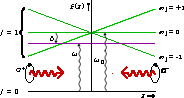
\includegraphics[width=\linewidth]{figures/OpticalMolasses.pdf}
	\end{minipage}
	\begin{minipage}{.48\textwidth}
		\centering
		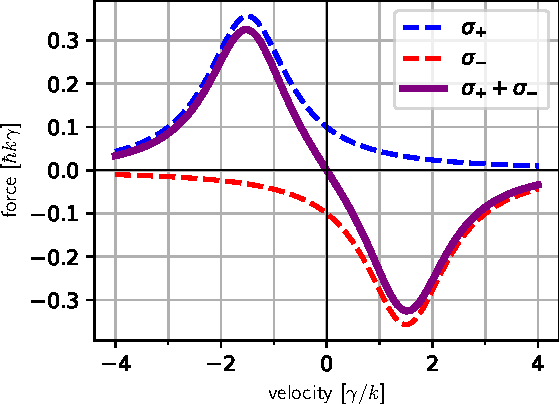
\includegraphics[width=\linewidth]{figures/MOTplot.pdf}
	\end{minipage}
	\caption{a) Concept of optical molasses in 1D. Atomic frequency is detuned from the atomic transition by $\delta<0$. Because of the linear magnetic field, at some displacement, the $m_j=-1$ atoms become resonant with only $\sigma^+$ light because of selection rules, and vice versa. b) Cooling force from a magneto-optical trap. Contributions from the $F^+$, $F^-$ and the total force are shown for $\delta = -\gamma$ and $I/I_0 = 2.$}
		\label{fig:MOTdamping}
\end{figure}

\begin{equation}\label{eq:linearize}
	F \approx - \hbar k^2 s_0 \frac{-2\delta/\gamma}{\left[1+s_0+(2\delta/\gamma)^2\right]^2} \equiv -\beta v
\end{equation}

Where $\beta$ is the slope of the scattering force around $v=0$. The resulting force has a dampening character on the velocity, which if applied in all 3 dimensions can effectively cool atoms. 

The treatment so far would suggest that this can be used to cool atoms to temperatures of absolute zero. This is not the case, as the random character of the scattering force means the atom fluctuates around the equilibrium velocity according to a Brownian motion. For $\delta=-\gamma/2$, $\beta$ is at a maximum, yielding the lowest possible temperature achievable using Doppler cooling called the Doppler temperature $T_D$

\begin{equation}\label{eq:DopplerTemperature}
	T_D = \frac{\hbar}{2k_b} \gamma.
\end{equation}

where $k_b$ is Boltzmann's constant. Apparently, this cooling limit is only dependent on the linewidth of the transition $\gamma$, apart from physical constants. This result will be used later in \cref{sec:Sr}.

\subsection{Magnetic Trapping}

Apart from cooling the atoms, we want to trap them at a specific location to increase the density of atoms. We can use the Zeeman effect for this, which tells us the atomic energy levels will be split an amount $\Delta E$ according to \cite{Griffiths2004}

\begin{equation}\label{eq:Zeeman}
	\Delta E = \mu_{\emph{B}} g_J m_j B,
\end{equation}

where $B$ is the Bohr magneton, $g_J$ the Landé g-factor, $m_j$ is the magnetic quantum number and $B_{\text{ext}}$ the applied magnetic field. The magnetic field is tuned in such a way that it is linear in all 3 dimensions and zero at the center of the \ac{MOT} by using a set of magnetic field coils in an anti-Helmholtz configuration. Because of the Zeeman splitting, the chance of the atoms coming in resonance with the laser varies with the position from the origin according to 

\begin{equation}\label{eq:DetuningFull}
	\delta' = \delta + k v - \frac{\mu'B}{\hbar}
\end{equation}

To ensure that atoms only absorb momentum kicks in the right direction, the laser beams are circularly polarized: $\sigma^+$ from the left and $\sigma^-$ from the right. Because the sign of the Zeeman shift is dependent on the magnetic quantum number $m_j$, selection rules prescribe. For 3 dimensions the force becomes

\begin{equation}\label{eq:MOTfull}
	\frac{F}{\hbar k \gamma s_0} = \frac{1}{2}\left\{\
	\left[1 + s_0 + 4\frac{(\delta+kv+\mu'B/\hbar)^2}{\gamma^2}\right]^{-1}+
	\left[1 + s_0 + 4\frac{(\delta-kv-\mu'B/\hbar)^2}{\gamma^2}\right]^{-1}
	\right\}
\end{equation}

Where $\mu' = (g_e m_e-g_g m_g)\mu_B$ is the effective magnetic moment for the transition \cite{Kowalski2010}. Expanding \cref{eq:MOTfull} around $(v,z) = (0,0)$, keeping only first order terms, extending the same concept to the other two dimensions yields finally

\begin{equation}\label{eq:ForceMOT}
	F_{\text{MOT}}(z,v) \approx -\beta v - \kappa z.
\end{equation}

Where $\beta$ is the same we found in \cref{eq:linearize} and $\kappa \equiv \mu' \beta /\hbar k \cdot \partial B/\partial z$. Apart from the dampening force, a force with Hookian character arises for linear magnetic field gradient as well. These are the two ingredients for producing high-density cold atom clouds. 



\section{Strontium}\label{sec:Sr}

Historically, people started laser cooling experimentation on group 1 or alkali atoms (Na, Rb, Cs). Because they only have one valence electron, the level structure is relatively straightforward. Also, diode lasers are available for their transition frequencies. This work is on the trapping of alkali earth atoms explained in \cref{ch:implementation}.

However, also group 2 atoms, also called alkali-earth (and similar atoms like Yb) are possible candidates. Because of their two valence electrons, the level structure is much more complicated, making laser cooling harder, but possibly also opening up new possibilities. The element we wish to use for our new machine in Eindhoven is Sr. For more extensive coverage of Sr, the reader is referred to \cite{Stellmer2013}. Three of them are bosonic, with ${}^{88}$Sr being the most abundant at $\sim82.6\%$. There is one stable fermionic isotope: ${}^{87}$Sr has a nuclear spin of $I=9/2$ and an abundance of $\sim7.0\%$ \cite{Coursey1999}. This work is on \textsuperscript{88}Sr. Because of the lack of hyperfine structure, it simplifies a whole lot of things, but in principle, one can work on all isotopes in the same machine as the energy splitting between the isotopes is in the MHz regime. 

Strontium is also used in the best atomic clocks in the world \cite{Bloom2014}, for some of the same reasons that it is a good candidate for quantum computing, which we will discuss here. 

\subsection{Relevant Transitions}

A simplified version of the level diagram of \textsuperscript{88}Sr is shown in \cref{fig:SrLevel}. The notation is $(n_1l_1 n_2l_2)^{2S+1}L_J$ where $n_{1,2}$ is the principal and $l_{1,2} = s, p, d, \ldots$ the azimuthal quantum number. Furthermore $S$, $L$ and $J$ are the total spin, orbital angular momentum, and total angular momentum respectively \cite{Cowan1981}.  This level scheme shows 6 out of 7 lasers to be used in this experiment. 

\begin{itemize}
	\item 461 nm. Broad transition, meaning a strong scattering force (\cref{eq:ScatteringFrequency} and short lifetime and quick cycling frequency. This is useful to slow down the hot atomic beam coming from the oven, as well as catching the atoms in a so-called blue \ac{MOT} with 'hot' temperatures of $\sim$ 1 mK.)
	
	\item 689 nm. Being much narrower than the blue transition, its Doppler temperature \cref{eq:DopplerTemperature} is much lower at $179$ nK, although in practice cooling is limited by the recoil limit to some $\sim 1$ $\mu$K \cite{Boyd2007,Stellmer2013}.
	
	\item 698 nm. The ultra-narrow clock transition ($\gamma = 1$ mK). Used in atomic clocks because of its spectroscopic accuracy \cite{Bloom2014}. It will turn out that this feature can be put to good use in quantum computers as well, and we will use it to coherently 'drive' the qubits between the qubit basis states. More about this in \cref{sec:QubitScheme}
	
	\item 679, 688, and 707 nm. All repump lasers. 707 and 688 are used to cycle back atoms from ending up in ${}^3P_2$ from the decay channel shown by the grey dotted line in \cref{fig:SrLevel}. 679 is used to prevent repump leaks to ${}^3P_0$ \cite{Stellmer2013,Xu2003}.
\end{itemize}

One wavelength is not shown, which is the laser that will supply the most amount of power. This is the trapping laser, which determines the number of single atoms and therefore qubits the machine can house. Using 813 nm, it is detuned so far from resonance that is not shown in \cref{fig:SrLevel} This wavelength gives the same light shift for ${}^1S_0$ and ${}^3 P_0$. This will be explained more thoroughly in \cref{sec:OpticalDipoleTrap}. 

\begin{figure}
	\centering
	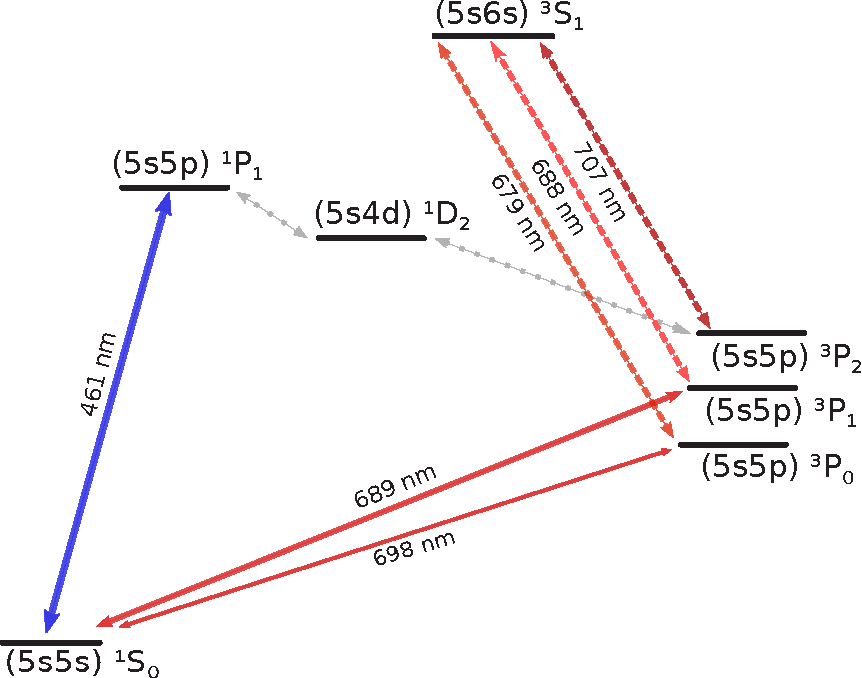
\includegraphics[width=0.55\linewidth]{figures/SrLevel.pdf}
	\caption{Simplified level scheme for \textsuperscript{88}Sr. Shown: blue transition for initial slowing and cooling. Narrower 689 nm transition of the red \ac{MOT}, and the \textsuperscript{1}S\textsubscript{0} - \textsuperscript{3}P\textsubscript{0} clock transition, which we will be used to drive the qubits. To increase density and trap lifetime 3 repump lasers are used. Not shown: 813 nm dipole trapping laser because it is driven far off-resonant. Energies not to scale. Figure made by Ivo Knottnerus.}
	\label{fig:SrLevel}
\end{figure}

\subsection{Laser Cooling and Trapping of Sr}

Because the melting temperature of Sr is $777$ ${}^{\circ}$C, to get any relevant vapor pressure, the Sr is heated in an oven after which it sublimates. To obtain a small atomic beam divergence, the atoms are directed along a bundle of high aspect ratio capillary tubes\cite{Stellmer2013}. 

Because of the oven, the atoms are moving way too fast to be efficiently captured by the MOT. Therefore, they are slowed by a Zeeman slower. This is a device similar to a MOT but designed to cool only in one direction. A red-detuned laser is propagating in the opposite direction of the atomic beam. A spatially varying magnetic field ensures a wide range of velocities is at some point resonant with the laser according to \cref{eq:DetuningFull}. 

Depending on the length of the Zeeman slower, only a fraction of the atoms will be slowed. To separate the hot from the cool atoms (the former are unwanted in a vacuum chamber) a deflection stage is used. The blue transition of Sr is used for this stage because of the strong scattering force. The Zeeman slowing and deflection stage is explained more elaborately in the thesis of Rik van Herk \cite{Herk2022}.

After the deflection stage, the atomic beam enters a glass cell. The advantage of using a glass cell is that it allows for the maximum amount of optical axis. To allow for longer trap survival times, the glass cell has \ac{UHV} which is separated from the stages preceding it by a differential pumping stage. 

\begin{figure}
	\centering
	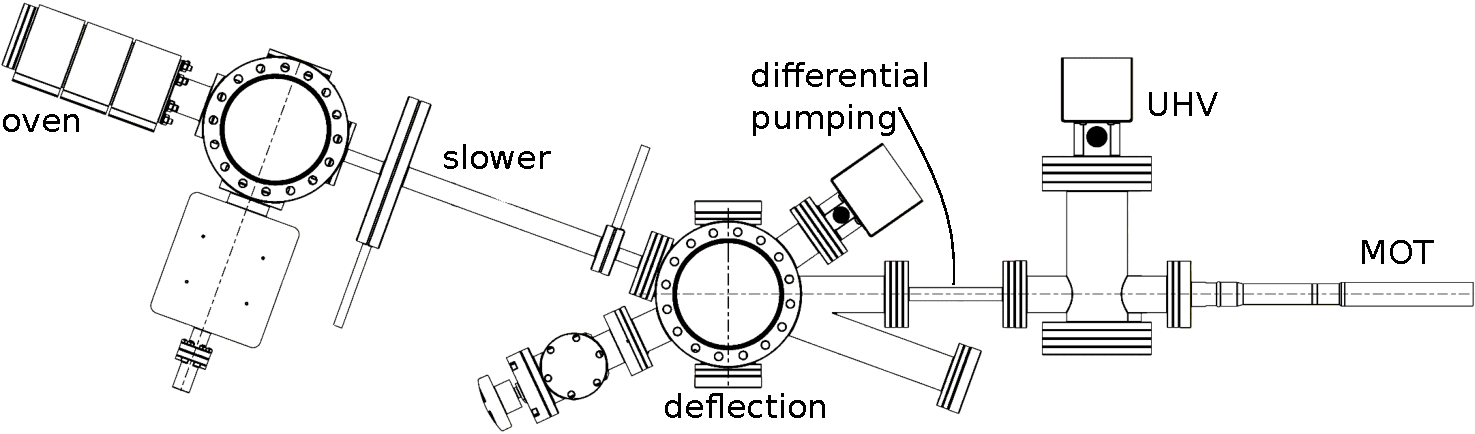
\includegraphics[width=0.9\linewidth]{figures/SrLoading.pdf}
	\caption{Sketch of the vacuum atom source design and vacuum chambers. Starting from the oven, the atomic beam traverses a Zeeman slower, deflection stage, and differential pumping stage before ending in the glass cell (MOT, right). Figure by Patrick de Laat.}
	\label{fig:SrLoading}
\end{figure}

\subsection{Strontium as a Qubit}\label{sec:QubitScheme}

The main reason we want to use strontium atoms for the quantum processing unit is the ${}^3P_0$ state and its very long lifetime. The clock transition is forbidden according to selection rules and only opens up after applying a magnetic field for the \textsuperscript{88}Sr isotope, after which the lifetime is in the order of $\sim 100$ s. On the timescales of the operation of a quantum computer, we can therefore consider ${}^3P_0$ a 'second ground state'. 

We aim to define the two clock states as our qubit manifold, such that we have:

\begin{equation}\label{eq:QubitManifold}
	\big\{\ket{0},\ket{1}\big\} = 
	\left\{
		\ket{{}^1S_0}, \ket{{}^3P_0} 
	\right\}
\end{equation}

Such that we have two long-lifetime states with an extremely narrow transition between them such that we can coherently drive between the qubit states. Because both states are 'ground' states, this type of scheme is called $\ket{gg}$ \cite{Wu2021}. To entangle the qubits, Rydberg dressing can be used \cite{Wu2021} where a small part of a Rydberg state $\ket{r}$ is admixed in one of the ground states. 

\begin{equation}\label{eq:RydbergDressing}
	\ket{\psi} \sim \ket{g} + \epsilon \ket{r}
\end{equation}

The degree dressing is tuned by the (small) dressing parameter $\epsilon \propto \Omega / 2\delta$ where $\Omega$ is the Rabi frequency of the laser and $\delta$ the usual detuning. A Rydberg state is an electronic state with a very high principal quantum number $n$. Rydberg atoms are physically larger, as the electron orbit scales $\propto n^2$ \cite{Gallagher1994}. As a result of these exaggerated electron orbit sizes, neighboring atoms can 'feel' each other. For example, the van der Waals interaction coefficient scales as $\propto n^{11}$ \cite{Gallagher1994}. 

Other qubit implementations than the one above are possible as well. For example, \cite{Barnes2021} uses the fermionic ${}^{87}$Sr and maps the qubit states onto the nuclear spin states $\ket{{}^1S_0, F=9/2, m_F = -9/2}$ and $\ket{{}^1S_0, F=9/2, m_F = -7/2}$ nuclear magnetic spin states. 


\section{Optical Dipole Traps}\label{sec:OpticalDipoleTrap}

Now that the qubit manifold is known, we will talk about how to experimentally trap these qubits. While magneto-optical traps are excellent for producing clouds of ultracold atoms, the constant photon scattering is unwanted during qubit operation. Therefore, after the atom cloud is cooled in the \ac{MOT}, the MOT is typically overlapped with another type of trap: \ac{ODT}. An ODT uses far-off-resonant light and is therefore much weaker. However, because the light is off-resonant, such that scattering events are kept to a minimum and are thus non-destructive for coherence. 

The light field $\mathbf{E}$ will induce a dipole moment $\mathbf{p}$ in the atom according to 
	
\begin{equation}\label{eq:DipoleMoment}
	\mathbf{p} = \alpha \mathbf{E}
\end{equation}

in turn, the dipole potential will interact with the electric field leading to and an interaction dipole potential $U_{dip}$

\begin{equation}\label{eq:DipolePotential}
	U_{\text{dip}}(\mathbf{r}) = -\mathbf{p}\mathbf{E} = 
	-\frac{1}{2} \left\langle \mathbf{p}\mathbf{E} \right\rangle = \frac{\operatorname{Re}(\alpha)}{2\epsilon_0 c} I(\mathbf{r})
\end{equation}

where we have averaged the rapidly oscillating phase terms of the light, giving the factor $1/2$ and furthermore $I(\mathbf{r}) = |\mathbf{E}(\mathbf{r})|^2/(2\epsilon_0 c)$ where $\epsilon_0$ is the electric constant. The dipole force thus scales with the in-phase part of the polarizability with the light field. An additional factor $1/2$ comes in because the dipole moment is induced and not permanent. The gradient of \cref{eq:DipolePotential} gives rise to the dipole force:

\begin{equation}\label{eq:DipoleForce}
	\mathbf{F}_{\text{dip}}(\mathbf{r}) = - \frac{\operatorname{Re}(\alpha)}{2\epsilon_0c}\nabla I(\mathbf{r})
\end{equation}

\cref{eq:DipoleForce} tells us that to maximize the dipole force, one has to maximize the gradient of the light intensity profile. This can be done by focussing the laser on the smallest possible spot, to achieve the highest possible dipole force. The scattering rate from the ODT can be found by averaging over the derivative of the dipole moment with the electric field 

\begin{equation}\label{eq:ScatteringRate}
	\Gamma_{\text{sc}}(\mathbf{r}) = \frac{\left\langle \mathbf{p} \mathbf{E} \right\rangle}{\hbar \omega}
	 = \frac{\operatorname{Im}(\alpha)}{\hbar \epsilon_0 c} I(\mathbf{r}) 
\end{equation}

These expressions are true for any atom in a potential. The fact that $\alpha$ is complex means there is a phase delay between the electric field and the dipole response. The task that remains is finding the polarizability $\alpha$. As a starting point, we will consider the electron as a harmonic oscillator with a damping coefficient. The dampening yields the polarizability, which for alkali atoms like Rb is accurate to within a few percent: 

\subsection{Classical}

In the classical picture, we assume a classical light field, as well as a classical electron (harmonic oscillator). We can write down a general expression for the the light field propagating in the $z$-direction polarized in the $\bm{\hat{\epsilon}}$ direction perpendicular to it:

\begin{equation}\label{eq:ClassicalField}
	\mathbf{E}(z,t) = \mathbf{E}_0 \cos{(k z - \omega t)} 	\bm{\hat{\epsilon}}
\end{equation}
	 
The electron is modeled as a damped harmonic oscillator (Lorentz oscillator). Integrating the equation of motion for the electron, assuming a dipole moment $\mathbf{p} = e \mathbf{r}$ where $r$ is the position yields after equating to \cref{eq:DipoleMoment} for the polarizability \cite{Grimm2000}

\begin{equation}\label{eq:LorentzOscillator}
	\alpha=6 \pi \epsilon_{0} c^{3} \frac{\Gamma / \omega_{0}^{2}}{\omega_{0}^{2}-\omega^{2}-\mathrm{i}\omega^3\Gamma/\omega_0^2}
\end{equation},

Where $\Gamma$ is the on-resonant damping rate in terms of the electron mass $m_e$. 

\begin{equation}\label{eq:ResonantDampingRate}
	\Gamma = \frac{e^2 \omega_0^2}{6\pi \epsilon_0 m_e c^3}
\end{equation}

Inserting \cref{eq:LorentzOscillator} in \cref{eq:DipolePotential,eq:ScatteringRate} yields, after assuming $\delta \ll \omega, \Gamma \ll \omega$

\begin{equation}\label{eq:DipoleClassicalResult} 
	U_{\text{dip}}(\mathbf{r}) = 
	\frac{3\pi c^2}{2\omega_0^3}\frac{\Gamma}{\delta} I(\mathbf{r}),
	\quad
	\Gamma_{\text{sc}}(\mathbf{r}) = 
	\frac{3\pi c^2}{2\hbar\omega_0^3}\left(\frac{\Gamma}{\delta}\right)^2 I(\mathbf{r})
\end{equation}

The two parameters that we can control are the light intensity $I(\mathbf{r})$ and the detuning $\delta$ \cite{Grimm2000}. The relationship between them is $\hbar \Gamma_{sc} =\Gamma U_{\text{dip}}/\delta$. So to keep scattering events to a minimum and obtain deep traps, we should use large detunings. To ensure the traps are deep, high light intensities are used. 

\subsection{Semi-Classical}

In the semi-classical picture, we consider the same classical light field \cref{eq:ClassicalField}, but consider an atom with quantized energy levels. We will consider a two-level atom with eigenstates $\ket{g}$ (ground) with energy $\hbar \omega_g$ and $\ket{e}$ (excited) with $\hbar \omega_e$,see \cref{fig:2LevelAtom}. Then the atomic Hamiltonian in this basis reduces to \cite{Loudon2000}

\begin{figure}
	\centering
	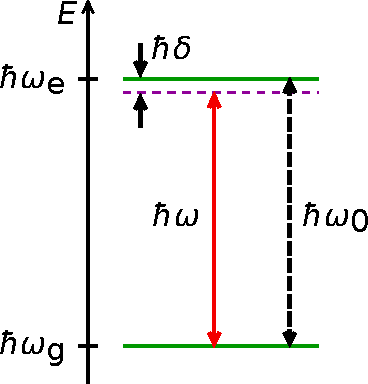
\includegraphics[height=4.1cm]{figures/2LevelAtom.pdf}
	\caption{Energy level scheme for the 2-level case. The two energies are split by $\omega_e - \omega_g = \omega_0$. The detuning is $\delta = \omega-\omega_0$.}
	\label{fig:2LevelAtom}
\end{figure}

\begin{equation}\label{eq:AtomHamiltonianMain}
	\mathcal{H}_A = \hbar \omega_g \ket{g}\bra{g} + \hbar \omega_e \ket{e}\bra{e}
\end{equation}

The radiation field is modeled as a time-dependent perturbation such that the total Hamiltonian is \cite{Leeuwen2017}

\begin{equation}\label{eq:PerturbationMain}
	\mathcal{H} = \mathcal{H}_A + \mathcal{H}_{I}(t),
\end{equation}

We can write down the wave function in the basis of the atomic eigenstates, and their time evolution is now given by

\begin{equation}\label{eq:TwoLevelMain}
	\ket{\psi} = c_g(t) e^{-i \omega_g t} \ket{g} + c_e(t) e^{-i \omega_e t} \ket{e}.
\end{equation}

In appendix \ref{ch:LightMatter} the Schrodinger equation is solved for the 2-level atom using the dipole approximation as well as the \acf*{RWA}. The following matrix equation is derived for the 2 level atom (\cref{fig:2LevelAtom}) \cite{Foot2005}

\begin{equation}\label{eq:MatrixEvolution}
	i \hbar \begin{pmatrix}
		\dot{c}_g \\ 
		\dot{c}e
	\end{pmatrix}
	= \frac{\hbar}{2} \begin{pmatrix}
		\delta & \Omega \\ \Omega^* & -\delta 
	\end{pmatrix} 
	\begin{pmatrix}
		c_g \\ c_e
	\end{pmatrix}
\end{equation}.

where the coupling between the atomic eigenstates and the radiation field is described by the Rabi frequency:

\begin{equation}\label{eq:RabiFrequencyMain}
	\Omega \equiv \frac{e E_0}{\hbar} \bra{g}\mathbf{r}\ket{e}
\end{equation}

The Hamiltonian of \cref{eq:MatrixEvolution} has eigenvalues 

\begin{equation}\label{eq:EigenValues}
	E_{\pm} = \pm
	\frac{\hbar}{2} \sqrt{\Omega^2+\delta^2}
\end{equation}. Assuming $|\delta| \gg \Omega$, the eigenenergies are thus 

\begin{equation}
	E_g =  \frac{\hbar \delta}{2} +\frac{\hbar \Omega^2}{4 \delta}, \quad
	E_e = -\frac{\hbar \delta}{2} -\frac{\hbar \Omega^2}{4 \delta}
\end{equation}

When turning on the laser, the energies are thus shifted by an amount $\Delta E = E(\Omega)-E(\Omega=0)$ And it turns out the eigenenergies are shifted by an amount known as the light shift or AC stark shift \cite{Vredenbregt2020}. See \cref{fig:DipoleForce}.

\begin{figure}
    \centering
	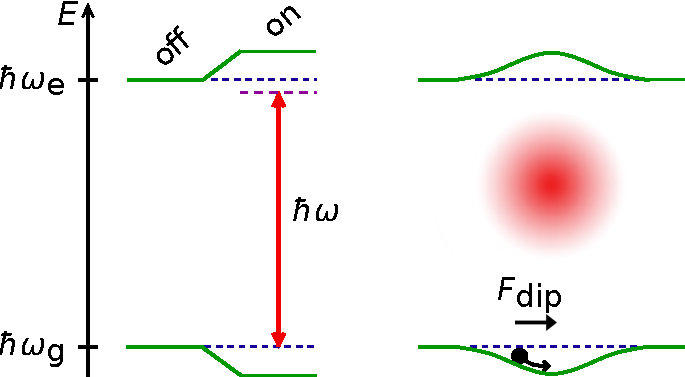
\includegraphics[height=3.8cm]{figures/LightShift.pdf}
	\caption{Light shift when the off-resonant laser is turned on, as well as the spatially varying light shift for a laser beam profile for $delta<0$.}
	\label{fig:DipoleForce}
\end{figure}

\begin{equation}\label{eq:Stark}
	\Delta E_{e,g} = \pm \frac{\hbar \Omega^2}{4 \delta}.
\end{equation}

The light shift is proportional to the light intensity over the detuning: $\Omega^2 / \delta \propto I / \delta$, which we already found for the classical treatment in \cref{eq:DipoleClassicalResult}. This behavior is shown in \cref{fig:DipoleForce}. Because the field is off-resonant, atoms only occupy the ground state. For $\delta <0$ ('red detuned'), the ground state light state is negative. To calculate the new eigenstates, we repeat the treatment for a quantized light field, known as the dressed state picture.

\subsection{Dressed Atom Approach}

To calculate the new shifted eigenstates, the full Hamiltonian has to be considered, included a quantized light field with Hamiltonian $\mathcal{H}_L$ \cite{Dalibard1985}

\begin{equation}
	\mathcal{H} = \mathcal{H}_A + \mathcal{H}_L + \mathcal{H}_I(t)
\end{equation}

where the light field has eigenenergies separated by the photon energy and eigenstates of $n$ photons: $\ket{n}$ \cite{Vredenbregt2020}

\begin{equation}
	\mathcal{H}_L = \sum_n \hbar \omega \left(n+\frac{1}{2}\right) \ket{n}\bra{n}
\end{equation}

The new eigenstates are 

\begin{equation}
	\begin{split}
		\ket{1} &= \cos{\theta} \ket{g,n} - \sin{\theta} \ket{e,n-1},\\
		\ket{2} &= \sin{\theta} \ket{g,n} + \cos{\theta} \ket{e,n-1}
	\end{split}
\end{equation}

where the mixing angle $\theta$ is $\cos{(2\theta)}=-\delta / \sqrt{\delta^2+\Omega^2}$


	

